\section{Análisis de los algortitmos}

Para analizar los 3 algoritmos estudiado Box Counting Fixed Size (BCFS), Box Covering Compact (BCC) y SandBox(SB); se seleccionan algunas redes de prueba, las cuales pueden ser consultadas en el Anexo A de la página \pageref{AnexoA},

La configuración y protocolo de pruebas es explicado en el Anexo B de la página\pageref{AnexoB}


\subsection{Redes libres de escala}

Se selecciona la red libre de escala de 4000 nodos 

Inicialmente, para cada estrategia se analiza la relación entre $q$ y $\ln(Zr(q))$

\begin{figure}[H]
    \centering
    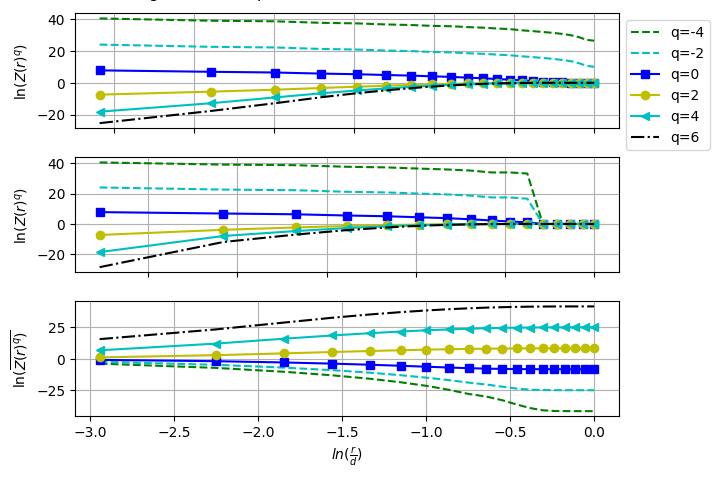
\includegraphics[scale=0.8]{Capitulo4Multifractalidad/imagenes/scaleFree4000_TqLnrBCscaleFree4000Nodes.png}

    \caption{Regresión lineal entre $\ln(Z_r(q)$ y $\ln(\frac{r}{b})$. De arriba hacia abajo, la primera figura corresponde al método BCFS, la segunda al método BCC y la tercera SB}
\end{figure}

Cada valor de $q$ tiene su función de la cual se obtiene su pendiente, la cual corresponde a sus exponentes de masa.

\begin{figure}[H]
    \centering
    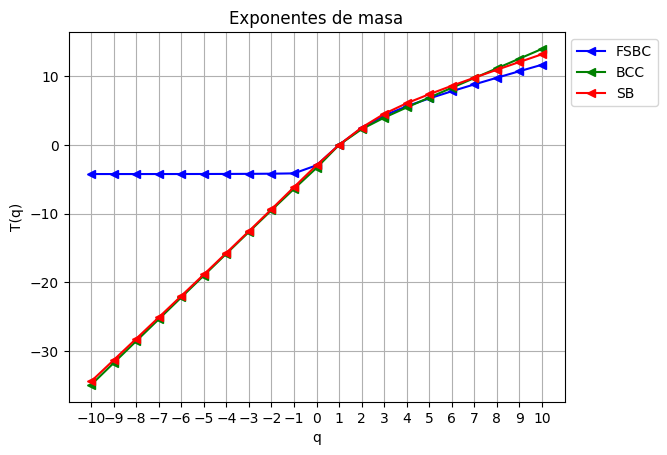
\includegraphics[scale=0.7]{Capitulo4Multifractalidad/imagenes/scaleFree4000_TqscaleFree4000Nodes.png}
    \caption{Exponentes de masa para red libre de escala 4000 nodos}
\end{figure}

Se observa que para el método BCFS los $q<0$ no tienen significado, esto se debe a que en cada caja se toma la cantidad de nodos sobre el total, lo que da valores menores que 1, al elevarlos a un valor $q$ se transforman en valores muy pequeños. Por esta razón, la dimensión se analiza para $q\geq0$

\begin{figure}[H]
    \centering
    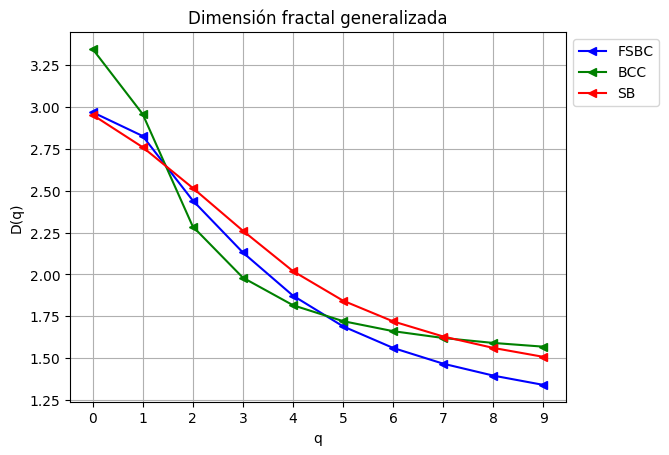
\includegraphics[scale=0.7]{Capitulo4Multifractalidad/imagenes/scaleFree4000_DqscaleFree4000Nodes.png}
    \caption{Dimensión fractal generalizada para red libre de escala 4000 nodos}
\end{figure}

De esta se puede obtener la siguiente información y compararla con el articulo de Wang\cite{Wang2012}:

\begin{table}[H]
    \centering
    \begin{tabular}{|c|c|c|c|c|}
        \hline
         \textbf{Dato}& \textbf{BCFS} & \textbf{BCC} & \textbf{SB} & \textbf{Articulo} \\
         \hline
         Dimensión fractal & 2.97 & 3.34 & 2.95 & 3.19 \\
         \hline
         Dimensión fractal generalizada & 2.82 & 2.95 & 2.75 &3.15  \\
         \hline
         Dimensión de correlación & 2.44 & 2.28 & 2.51 &2.81 \\
         \hline
         Dimensión máxima & 2.97 & 3.34 & 3.14 &3.26 \\
         \hline
         Dimensión mínima & 1.29 & 1.55 & 1.46 &1.75 \\
         \hline
         Variación en la dimensión & 1.68 & 1.79 & 1.68 &1.51 \\
         \hline
    \end{tabular}
    \caption{Comparación de los datos obtenidos con los del artículo de Wang\cite{Wang2012}}
\end{table}

Las diferencias en la medida de la dimensión fractal se deben a que el método es una aproximación y debe ejecutarse muchas veces, además que las redes del articulo y la generada son distintas.

Para evitar estas diferencias Li\cite{Li2014} recomienda que para el caso de $q=0$ se tome directamente la dimensión fractal obtenida por algoritmo de Box Counting, que en este caso es 3.13.

En las gráficas se puede observar que las redes libres de escala son multifractales, algo que es esperado ya que internamente estas redes tienen estructuras diferentes debido a la presencia de hubs altamente conectados.

\subsection{Redes de mundo pequeño}

A continuación se realiza el mismo proceso para una red de mundo pequeño con 5000 nodos generada con un modelo de Watts-Strogatz con una probabilidad de reconexión del 10\%

\begin{figure}[H]
    \centering
    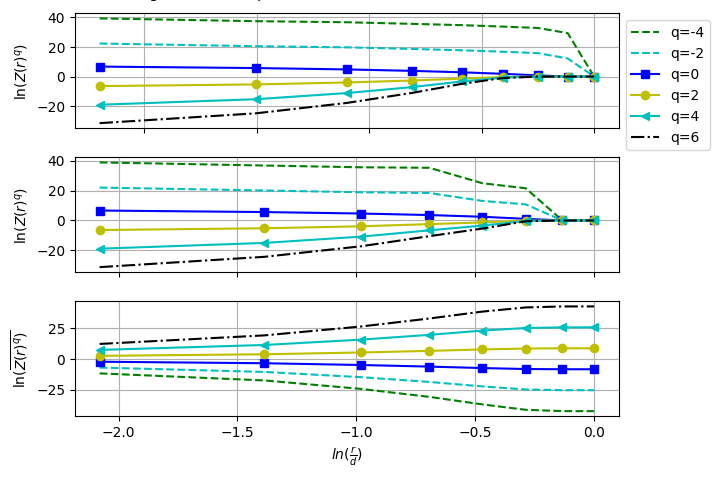
\includegraphics[scale=0.7]{Capitulo4Multifractalidad/imagenes/a_TqLnrBCsmallWorld4000p10.png}
    \caption{Regresión lineal entre $\ln(Z_r(q)$ y $\ln(\frac{r}{b})$. De arriba hacia abajo, la primera figura corresponde al método BCFS, la segunda al método BCC y la tercera SB}
\end{figure}

A continuación, los exponentes de masa:


\begin{figure}[H]
    \centering
    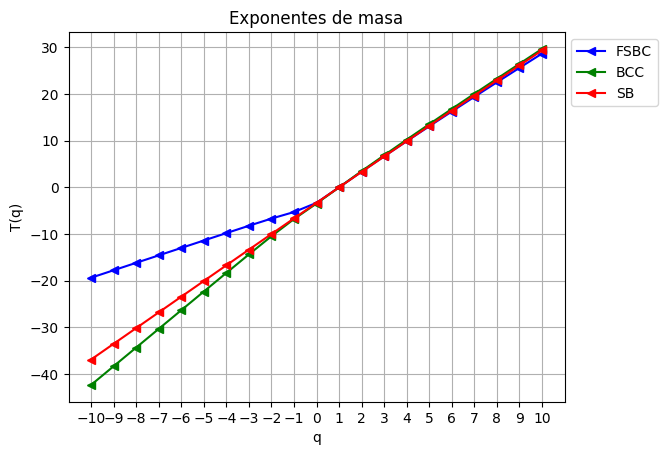
\includegraphics[scale=0.7]{Capitulo4Multifractalidad/imagenes/a_TqsmallWorld4000p10.png}
    \caption{Exponentes de masa para red de mundo pequeño con 5000 nodos y $p=10\%$}
\end{figure}

Finalmente, la dimensión fractal generalizada


\begin{figure}[H]
    \centering
    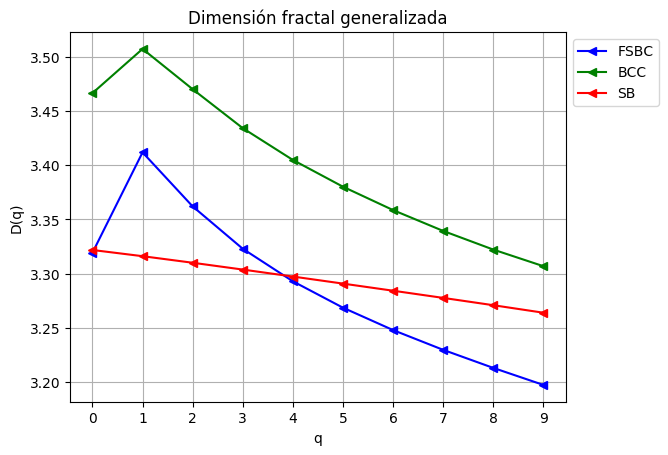
\includegraphics[scale=0.7]{Capitulo4Multifractalidad/imagenes/a_DqsmallWorld4000p10.png}
    \caption{Dimensión fractal generalizada para red de mundo pequeño con 5000 nodos y $p=10\%$}
\end{figure}

De acuerdo a los datos del articulo se encuentra:


\begin{table}[H]
    \centering
    \begin{tabular}{|c|c|c|c|c|}
        \hline
         \textbf{Dato}& \textbf{BCFS} & \textbf{BCC} & \textbf{SB} & \textbf{Articulo} \\
         \hline
         Dimensión fractal &3.31 & 3.46 & 3.32 & 2.79 \\
         \hline
         Dimensión fractal generalizada & 3.41 & 3.5 & 3.31 &2.8  \\
         \hline
         Dimensión de correlación & 3.36 & 3.47 & 3.31 &2.81 \\
         \hline
         Dimensión máxima & 3.41 & 3.84 & 3.35 &2.81 \\
         \hline
         Dimensión mínima & 3.18 & 3.29 & 3.25 &2.75 \\
         \hline
         Variación en la dimensión & 0.23 & 0.55 & 0.1 &0.06 \\
         \hline
    \end{tabular}
    \caption{Comparación de los datos obtenidos con los del artículo de Wang\cite{Wang2012}}
\end{table}

Los resultados varían ya que las redes del articulo y las utilizadas en estas pruebas son generadas, es decir que no son las mismas.

Se observa que la variación en la dimensión fractal es pequeña, de hecho menor que 1, por lo que, se puede concluir que las redes de mundo pequeño son monofractales, es decir que se pueden considerar como una sola estructura. Es importante indicar que las mediciones de los diferentes algoritmos requieren un mayor número de iteraciones para mejorar su presición.

La dimensión fractal de esta red es 3.47

\subsection{Redes aleatorias}

Se selecciona la red aleatoria de 5620 nodos.

\begin{figure}[H]
    \centering
    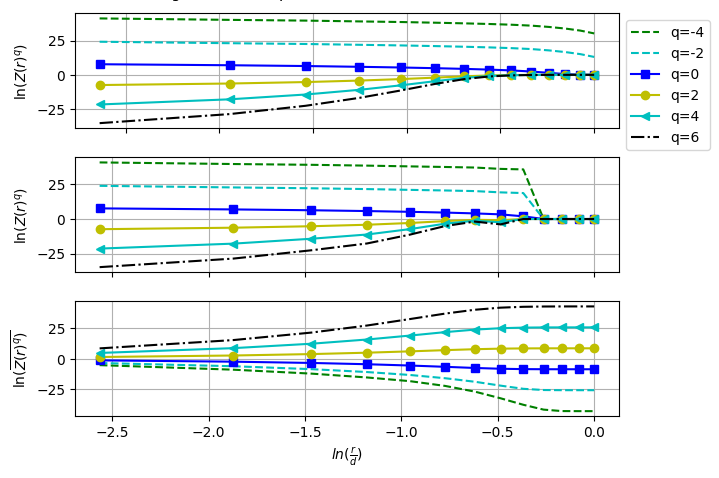
\includegraphics[scale=0.7]{Capitulo4Multifractalidad/imagenes/a_TqLnrBCrandom5620.png}
    \caption{Regresión lineal entre $\ln(Z_r(q)$ y $\ln(\frac{r}{b})$. De arriba hacia abajo, la primera figura corresponde al método BCFS, la segunda al método BCC y la tercera SB}
\end{figure}

\begin{figure}[H]
    \centering
    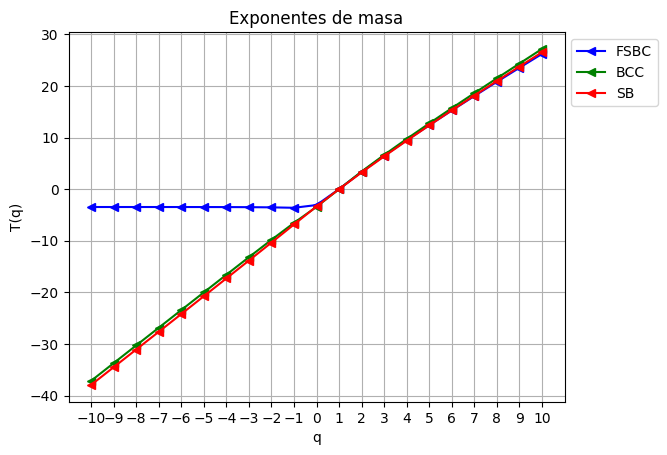
\includegraphics[scale=0.7]{Capitulo4Multifractalidad/imagenes/a_Tqrandom5620.png}
    \caption{Exponentes de masa para red aleatoria de 5620 nodos}
\end{figure}

\begin{figure}[H]
    \centering
    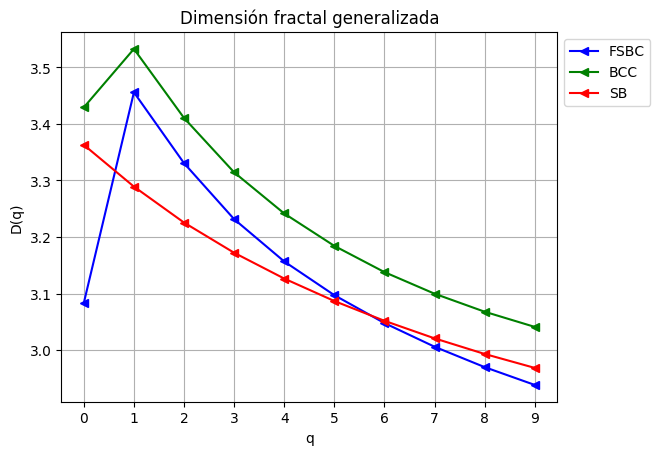
\includegraphics[scale=0.7]{Capitulo4Multifractalidad/imagenes/a_Dqrandom5620.png}
    \caption{Dimensión fractal generalizada para para red aleatoria de 5620 nodos}
\end{figure}

La dimensión fractal de esta red es: 3.41

Los análisis realizados a las redes de prueba, permite concluir que el análisis multifractal no permite caracterizar redes aleatorias, ya que pueden presentar comportamiento monofractal o multifractal. En este caso la red puede considerarse monofractal.

\begin{table}[H]
    \centering
    \begin{tabular}{|c|c|c|c|c|}
        \hline
         \textbf{Dato}& \textbf{BCFS} & \textbf{BCC} & \textbf{SB} & \textbf{Articulo} \\
         \hline
         Dimensión fractal & 3.08 & 3.42 & 3.36 & 3.54\\
         \hline
         Dimensión fractal generalizada  & 3.46 & 3.53 & 3.28 & 3.56 \\
         \hline
         Dimensión de correlación & 3.33 & 3.41  & 3.22 &3.52 \\
         \hline
         Dimensión máxima & 3.45 & 3.53 & 3.46 & 3.54\\
         \hline
         Dimensión mínima & 3.08 & 3.01 & 2.94 & 3.61\\
         \hline
         Variación en la dimensión & 0.37 &  0.52 & 0.52 & 0.33 \\
         \hline
    \end{tabular}
    \caption{Comparación de los datos obtenidos con los del artículo de Wang\cite{Wang2012}}
\end{table}



\subsection{Redes reales}

De las redes reales de prueba, se selecciona la red ECOLI.

\begin{figure}[H]
    \centering
    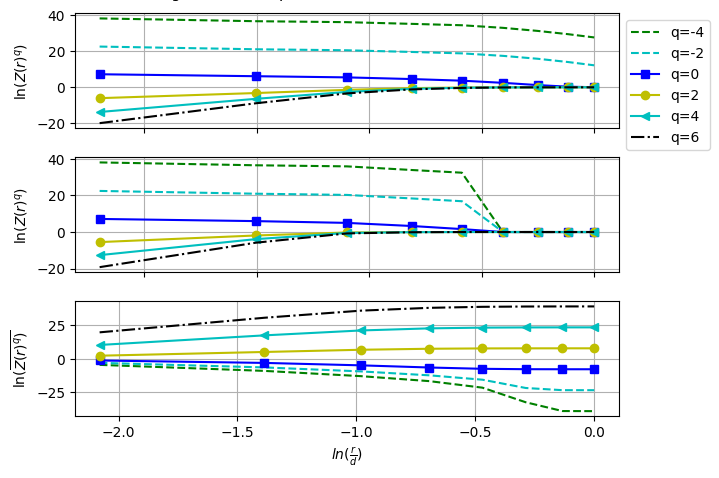
\includegraphics[scale=0.7]{Capitulo4Multifractalidad/imagenes/a_TqLnrBCecoli.png}
    \caption{Regresión lineal entre $\ln(Z_r(q)$ y $\ln(\frac{r}{b})$. De arriba hacia abajo, la primera figura corresponde al método BCFS, la segunda al método BCC y la tercera SB}
\end{figure}

\begin{figure}[H]
    \centering
    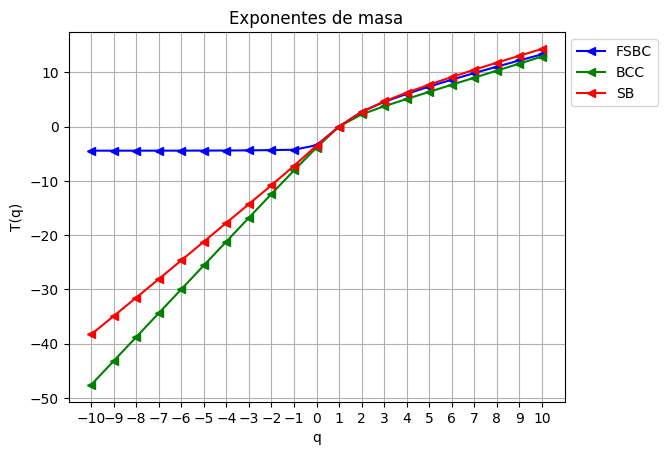
\includegraphics[scale=0.7]{Capitulo4Multifractalidad/imagenes/a_Tqecoli.png}
    \caption{Exponentes de masa para red real ecoli}
\end{figure}

\begin{figure}[H]
    \centering
    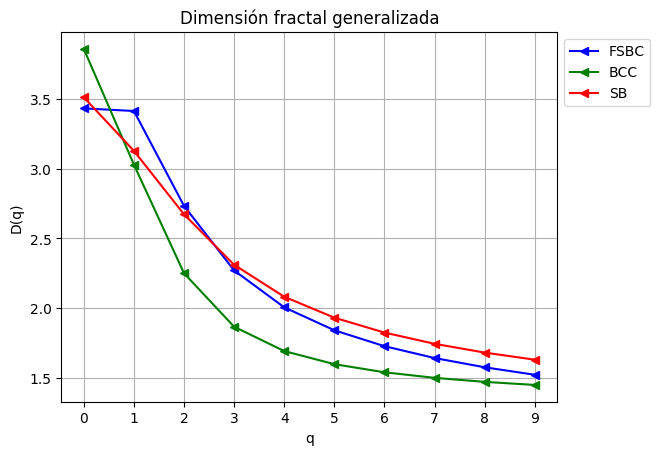
\includegraphics[scale=0.7]{Capitulo4Multifractalidad/imagenes/a_Dqecoli.png}
    \caption{Dimensión fractal generalizada para para red real ecoli}
\end{figure}

La dimensión fractal de esta red es 3.31

\begin{table}[H]
    \centering
    \begin{tabular}{|c|c|c|c|c|}
        \hline
         \textbf{Dato}& \textbf{BCFS} & \textbf{BCC} & \textbf{SB} & \textbf{Articulo} \\
         \hline
         Dimensión fractal & 3.43 & 3.35 & 3.51 & 3.56 \\
         \hline
         Dimensión fractal generalizada  & 3.41 & 3.03 & 3.12 & 3.45 \\
         \hline
         Dimensión de correlación & 2.73 & 2.25 & 2.67 & 2.9 \\
         \hline
         Dimensión máxima & 3.41 & 4.32 & 3.6 & 4.15 \\
         \hline
         Dimensión mínima & 1.47 & 1.43 & 1.5 & 2.1 \\
         \hline
         Variación en la dimensión & 1.94 & 2.91   & 2.1 & 2.05 \\
         \hline
    \end{tabular}
    \caption{Comparación de los datos obtenidos con los del artículo de Wang\cite{Wang2012}}
\end{table}


\subsection{Redes fractales}

Utilizando el articulo de Liu y otros\cite{Liu2015} se trabaja con la (2,2)-flower.

\begin{figure}[H]
    \centering
    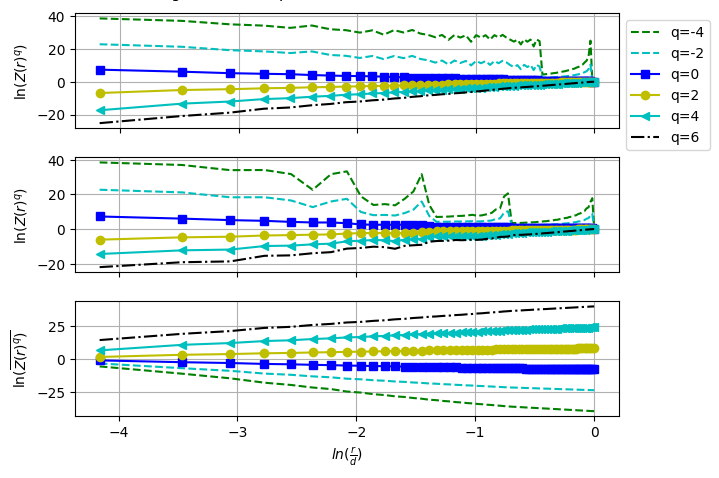
\includegraphics[scale=0.7]{Capitulo4Multifractalidad/imagenes/a_TqLnrBCflower22.png}
    \caption{Regresión lineal entre $\ln(Z_r(q)$ y $\ln(\frac{r}{b})$. De arriba hacia abajo, la primera figura corresponde al método BCFS, la segunda al método BCC y la tercera SB}
\end{figure}

\begin{figure}[H]
    \centering
    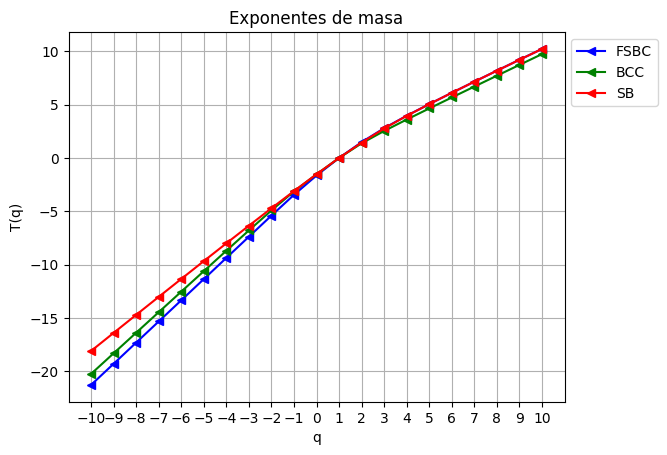
\includegraphics[scale=0.7]{Capitulo4Multifractalidad/imagenes/a_Tqflower22.png}
    \caption{Exponentes de masa para red real ecoli}
\end{figure}

\begin{figure}[H]
    \centering
    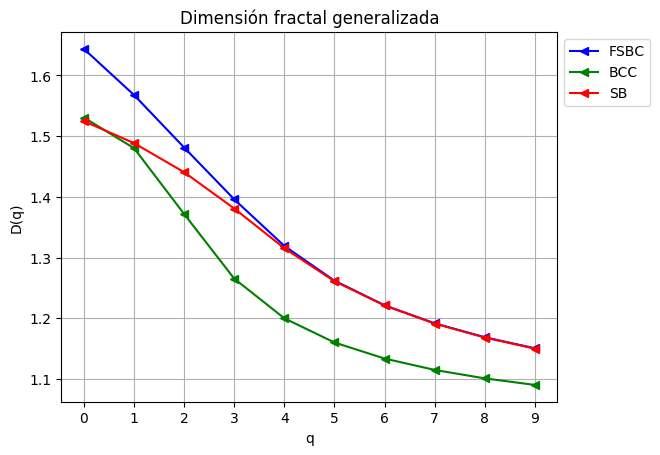
\includegraphics[scale=0.7]{Capitulo4Multifractalidad/imagenes/a_Dqflower22.png}
    \caption{Dimensión fractal generalizada para para red real ecoli}
\end{figure}

La dimensión fractal de esta red es 1.59


En el articulo sólo se realiza un análisis de gráficas, en el cual se indica que la red es levelmente multifractal. En en análisis del artículo se indica que la estructura en general es multifractal, ya que esta no es un fractal matemático, es decir que conserve su misma escala al infinito.

Los datos obtenidos de la red son.

\begin{table}[H]
    \centering
    \begin{tabular}{|c|c|c|c|}
        \hline
         \textbf{Dato}& \textbf{BCFS} & \textbf{BCC} & \textbf{SB} \\
         \hline
         Dimensión fractal & 1.64 & 1.53 & 1.52\\
         \hline
         Dimensión fractal generalizada  & 1.56 & 1.48 & 1.48\\
         \hline
         Dimensión de correlación & 1.48 & 1.37 & 1.44\\
         \hline
         Dimensión máxima & 1.92 & 1.83 & 1.64 \\
         \hline
         Dimensión mínima & 1.13 & 1.83& 1.13 \\
         \hline
         Variación en la dimensión & 0.79 & 0.74 & 0.51 \\
         \hline
    \end{tabular}
    \caption{Comparación de los datos obtenidos de los diferentes métodos de análisis multifractal}
\end{table}